\begin{center}
    \section{Grupos de homotopías}
\end{center}
\subsection{Homotopía}


Queremos asociar a cada espacio topológico $X$ un conjunto $h(X)$ que de preferencia tenga una estructura algebraica como grupo, grupo abeliano, $R$-módulo, etc., de modo que $h$ sea un invariante topológico, i.e., si tenemos espacios homeomorfos $X\cong Y$, entonces $h(X)\cong (Y)$ (isomorfos). 

Además, dada una función continua $f:X\to Y$, tenemos un homeomorfismo asociado $h(f):h(X)\to h(Y)$; con las siguientes propiedades
\begin{itemize}
    \item[(1)] $h(\id_X)=\id_{h(X)}$, \setlength{\parskip}{-0.3em}
    \item[(2)] Si $\begin{tikzcd}[column sep=0.5cm,row sep=1.25cm]  
                    X \ar[r,"f"] & Y \ar[r,"g"] & Z
                \end{tikzcd}$
            son funciones continuas, entonces $h(g\circ f)=h(f)\circ h(g)$,
\end{itemize}
\begin{nota}
    Si $h$ satisface (1) y (2), entonces $h$ es un invariante topológico, ya que si $X\cong Y$, entonces existe $f:X\to Y$, $g:Y\to X$ continuas tal que
    \[
    g\circ f=\id_X\;\text{ y }\; f\circ g=\id_Y,
    \]
    entonces por (1) y (2), tenemos
    \begin{equation*}
        h(g)\circ h(f)=h(g\circ f)=h(\id_X)=\id_{h(X)}
    \end{equation*}
    y también 
    \begin{equation*}
        h(f)\circ h(g)=h(f\circ g)=h(\id_Y)=\id_{h(Y)},
    \end{equation*}
    entonces $h(f)$ es un isomorfismo con inversa $h(g)$.

    Por otro lado, necesitamos métodos para calcular $h(X)$ y $h(f)$ para $f$ una función continua. Los invariantes básicos que se nos puede ocurrir es hablar de las componentes conexas, conectable por trayectoría, etc. En general, estos invariantes no tienen estructura de grupo, pero existen casos especiales en los que si resultan serlo, aunque no son triviales y por lo regular son \textit{muy difícil} de calcularlos.

    Por lo que respecta a este curso, solo hablaremos de componentes por trayectoría.
\end{nota}
\begin{definicion}
\label{rel:homo}
    Sea $X$ un espacio topológico. Definimos una relación en $X$ como sigue: sean $x,x'\in X$, decimos que $x\sim x'$ si existe $\sigma:I\to X$ (una trayectoria, con $I=[0,1]$) continua tal que $\sigma(0)=x$ y $\sigma(1)=x'$.
\end{definicion}

Veamos que está relación es de equivalencia. (1) Notemos que $x\sim x$, ya que $i:I\to X$ tal que $i(t)=x$, para toda $t\in I$, cumple con la definición $\ref{rel:homo}$. (2) Supongamos que $x\sim x'$, entonces existe una trayectoría continua $\sigma:I\to X$ tal que $\sigma(0)=x$ y $\sigma(1)=x'$. Consideremos la trayectoría $\overline{\sigma}:I\to X$ tal que $\overline{\sigma}(t)=\sigma(1-t)$, entonces $\overline{\sigma}$ es continua  y
\begin{align*}
    &\overline{\sigma}(0)=\sigma(1)=x',\\
    &\overline{\sigma}(1)=\sigma(0)=x,
\end{align*}
por lo tanto, $\overline{\sigma}$ es testigo de que $x'\sim x$. (3) Supongamos que $x_1\sim x_2$ y $x_2\sim x_3$, 
\[
\begin{tikzpicture}[x=1.5cm, y=0.7cm, font=\large]
  % Define point coordinates
  \coordinate (x1) at (0,0);
  \coordinate (x2) at (1.5,0);
  \coordinate (x3) at (3.5,0);

  % Draw horizontal ruled paper lines for context (optional, but good for positioning)
  %\foreach \i in {-1,0,1} \draw[lightgray, dashed] (-0.5,\i) -- (4,\i);

  % Draw the points (dots)
  \fill (x1) circle (1.8pt) node[below=3pt] {$x_1$};
  \fill (x2) circle (1.8pt) node[right=5pt] {$x_2$};
  \fill (x3) circle (1.8pt) node[right=3pt] {$x_3$};

  % Label for the terminal point
  %\node at (x3) {$x_3$};

  % Draw the path sigma (σ)
  \draw[thick, -, >=stealth] (x1) to[bend left=60] node[midway, yshift=1.5ex] {$\sigma$} (x2);

  % Draw the path tau (τ) - a wavy S-curve using explicit control points
  \draw[thick, -, >=stealth] (x2) .. controls ++(1,-2) and ++(-0.7, 1) .. (x3)
    node[near end, below=2pt, xshift=-1ex] {$\tau$};

\end{tikzpicture}
\]
tenemos entonces
\begin{equation*}
    \sigma(0)=x_1,\;\; \sigma(1)=\tau(0)=x_2\; \text{ y }\; \tau(1)=x_3.
\end{equation*}
Definamos $\sigma*\tau:I\to X$ como 
\begin{equation}
\label{producto entre trayectorias}
(\sigma * \tau)(t) = 
\begin{cases} 
\sigma(2t), & \text{si } 0 \leq t \leq \nicefrac{1}{2}; \\[1ex]
\tau(2t - 1), & \text{si } \nicefrac{1}{2} \leq t \leq 1. 
\end{cases}
\end{equation}
Notemos que $(\sigma*\tau)(\nicefrac{1}{2})=\sigma(1)=\tau(0)=x_2$, por lo que $\sigma*\tau$ está bien definida y además $I_1=[0,\nicefrac{1}{2}],\; I_2=[\nicefrac{1}{2},1]$ son conjuntos cerrados tal que $I=I_1\cup I_2$, por el lema del pegado, $\sigma*\tau$ es con- tinua. Finalmente 
\begin{align*}
    &(\sigma*\tau)(0)=\sigma(0)=x_1,\\
    &(\sigma*\tau)(1)=\tau(1)=x_3,
\end{align*}
por lo tanto, $\sigma*\tau$ es testigo de que $x_1\sim x_3$. 

%%% Comentario: La relación $\sim$ es de equivalencia, y denotamos por $[x]$ la clase de equivalencia de $x\in X$. El conjunto de todas las clases de equivalencia se denota por $\pi_0(X)$ y se llama el conjunto de componentes conexas por trayectorias de $X$.

%%% Más comentarios.
\begin{definicion}
    Denotamos por $\pi_0(X)$ el conjunto de clases de equivalencia que son las \textit{componentes por trayectoria} de $X$. Dado $x\in X$, su clase de equivalencia la denotamos por $\langle x\rangle \in \pi_0$(X). 
\end{definicion}
\begin{definicion}
\label{def: pi_0(f)}
    Sea $f:X\to Y$ una función continua, definimos $\pi_0(f):\pi_0(X)\to \pi_0(Y)$ tal que $\pi_0(f)(\langle x\rangle)=\langle f(x)\rangle$. Denotemos a $\pi_0(f)$ simplemente por $f_*$.
\end{definicion}
\begin{ejercicio}
    % ID: 1
    Mostrar que $f_*$ está bien definida y satisface que
    \begin{enumerate}[label=(\arabic*)]
        \item  ${\id_X}_*=\id_{\pi_0(X)}.$
        \item  Para cualquier $f:X\to Y$ y $g:Y\to Z$ funciones continuas, entonces $(g\circ f)_*=g_*\circ f_*$.
    \end{enumerate}
%\begin{dem}
%    Supongamos $x\simeq y$, entonces existe una trayectoría continua $\sigma:I\to X$ tal que $\sigma(0)=x$ y $\sigma(1)=y$. Entonces $f\circ \sigma(0)=f(x)$ y $f\circ \sigma(1)=f(y)$
%\end{dem}
\end{ejercicio}
\begin{coro}
    $\pi_0$ es un invariante topológico.
\end{coro}
\begin{definicion}
    Sea $X$ un espacio topológico y $x_0\in X$. Al par $(X,x_0)$ lo llamaremos \textit{espacio basado en} $x_0$.
\end{definicion}
\begin{definicion}
    Sea $X$ un espacio basado en $x_0$. Un \textit{lazo} con base en $x_0$ es una trayectoria continua $\alpha:I\to X$ tal que $\alpha(0)=\alpha(1)=x_0.$ Al conjunto de lazos en $X$ basado en $x_0$ lo denotamos por $\Omega(X,x_0).$
\end{definicion}
La deformación de lazos está dada por medio de una función continua $H:I\times I\to X$ llamada \textit{homotopía}, donde la primera coordenada del conjunto $I\times I$ denota el dominio de los lazos y la segunda coordenada denota el parámetro de la deformación que la podemos pensar como si fuese el \textit{tiempo}.
\begin{definicion}
\label{def:homotopia_relativa_lazos}
    Sea $\alpha,\beta\in \Omega(X,x_0)$, decimos que $\alpha$ se puede \textit{deformar} en $\beta$ o que $\alpha$ es \textit{homotópico} a $\beta$ y se denota por $\alpha \simeq\beta \rel$,  si existe una \textit{homotopía} $H:I\times I\to X$ que satisface lo siguiente:
    \begin{enumerate}
        \item $H(s,0)=\alpha(s)$, $H(s,1)=\beta(s)$.
        \item $H(0,t)=H(1,t)=x_0$.
    \end{enumerate}
\end{definicion}

La condición rel \{0,1\} es que los puntos $0,1\in I$ van a dar al mismo punto $x_0\in X$.

\begin{center}
\begin{tikzpicture}[
    scale=0.7, transform shape,
    % --- DEFINICIÓN DE ESTILOS ---
    % Estilo para poner una flecha en la parte superior del lazo
    midarrow/.style={postaction={decorate}, decoration={markings, mark=at position 0.32 with {\arrow{Stealth[length=2.5mm]}}}},
    % Estilos para los lazos
    alpha/.style={thick, blue!80!black, midarrow},
    beta/.style={thick, red!80!black, midarrow},
    % Estilo para los lazos intermedios
    inter/.style={thick, black, midarrow}
]

    % ==========================================
    % LADO IZQUIERDO: EL DOMINIO (Cuadrado I x I, tamaño 4 x 4)
    % ==========================================
    % Se ajustó el shift a (-8.0, -1.75) para que no choque con la flecha H al crecer
    \begin{scope}[shift={(-8.0, -1.75)}]
        
        % 4 Líneas horizontales simétricamente distribuidas (cada 0.8)
        \foreach \y in {0.8, 1.6, 2.4, 3.2} {
            \draw[inter] (0,\y) -- (4,\y);
        }

        % Bordes laterales (sin s=0 ni s=1)
        \draw[thick] (0,0) -- (0,4);
        \draw[thick] (4,0) -- (4,4);
        
        % Lazo alfa en el dominio (t=0)
        \draw[alpha] (0,0) -- (4,0) node[midway, below=2mm, font=\large, text=blue!80!black] {$t=0 \ (\alpha)$};
        
        % Lazo beta en el dominio (t=1)
        \draw[beta] (0,4) -- (4,4) node[midway, above=2mm, font=\large, text=red!80!black] {$t=1 \ (\beta)$};

        % Nombre del dominio en la parte superior, alineado perfectamente al nuevo centro
        \node[font=\Large] at (2, 5.5) {$I \times I$};
    \end{scope}

    % ==========================================
    % PARTE SUPERIOR: EL MAPEO HOMOTÓPICO (Flecha H)
    % ==========================================
    \draw[-{Stealth[length=3mm]}, thick] (-3.5, 2.5) to[bend left=20] node[above, yshift=1mm, font=\large] {$H$} (-1.2, 2.5);

    % ==========================================
    % LADO DERECHO: EL CODOMINIO (Espacio X)
    % ==========================================
    \begin{scope}[shift={(-0.7, 0)}]
        \node[font=\Large, text=black] at (2.5, 4.3) {$X$};
        % Frontera de X: Recorrida a la derecha (0.3 unidades), abrazando de cerca a los lazos pero respetando x_0
        \draw[thick, draw=black] (0.7, 0)
                                 .. controls (0.7, 1.8) and (-0.1, 3.8) .. (2.7, 3.8)
                                 .. controls (5.1, 3.8) and (5.7, 1.8) .. (5.7, 0)
                                 .. controls (5.7, -1.8) and (5.1, -3.8) .. (2.7, -3.8)
                                 .. controls (-0.1, -3.8) and (0.7, -1.8) .. cycle;

        \begin{scope}[shift={(1,0)}]
            
            % DIBUJAMOS DEL MÁS GRANDE AL MÁS CHICO
            
            % 1. Lazo beta (i=5) - El más externo y grande (ROJO)
            \pgfmathsetmacro{\L}{1.5 + 5*0.55}   % Longitud horizontal 
            \pgfmathsetmacro{\cx}{0.6 + 5*0.15}  % x del primer control
            \pgfmathsetmacro{\cy}{0.2 + 5*0.42}  % y del primer control
            \pgfmathsetmacro{\bx}{\L + 0.1 + 5*0.05} % x del segundo control
            \pgfmathsetmacro{\by}{0.9 + 5*0.7}   % y del segundo control 
            
            % Etiqueta \beta hacia AFUERA y abajo
            \draw[beta] (0,0) .. controls (\cx, \cy) and (\bx, \by) .. (\L, 0) 
                             .. controls (\bx, -\by) and (\cx, -\cy) .. (0,0) 
                             node[pos=0.5, right=6mm, yshift=4.5mm, font=\Large, text=red!80!black] {$\beta$};

            % 2. Lazos intermedios (i=4, 3, 2, 1) - (NEGROS)
            \foreach \i in {4, 3, 2, 1} {
                \pgfmathsetmacro{\L}{1.5 + \i*0.55}
                \pgfmathsetmacro{\cx}{0.6 + \i*0.15}
                \pgfmathsetmacro{\cy}{0.2 + \i*0.42}
                \pgfmathsetmacro{\bx}{\L + 0.1 + \i*0.05}
                \pgfmathsetmacro{\by}{0.9 + \i*0.7}

                \draw[inter] (0,0) .. controls (\cx, \cy) and (\bx, \by) .. (\L, 0) 
                                  .. controls (\bx, -\by) and (\cx, -\cy) .. (0,0);
            }

            % 3. Lazo alfa (i=0) - El más interno y pequeño (AZUL)
            \pgfmathsetmacro{\L}{1.5 + 0*0.55}
            \pgfmathsetmacro{\cx}{0.6 + 0*0.15}
            \pgfmathsetmacro{\cy}{0.2 + 0*0.42}
            \pgfmathsetmacro{\bx}{\L + 0.1 + 0*0.05}
            \pgfmathsetmacro{\by}{0.9 + 0*0.7}
            
            % Etiqueta \alpha
            \draw[alpha] (0,0) .. controls (\cx, \cy) and (\bx, \by) .. (\L, 0) 
                              .. controls (\bx, -\by) and (\cx, -\cy) .. (0,0) 
                              node[pos=0.5, right=3.5mm, font=\large, text=blue!80!black] {$\alpha$};

            % 4. Dibujar el punto x_0 por encima de todas las líneas para limpiar el origen
            \fill (0,0) circle (2.5pt) node[yshift=-0.5cm, font=\large] {$x_0$};
            
        \end{scope}
    \end{scope}

\end{tikzpicture}
\end{center}
\begin{ejercicio}
    % ID: 2
    Mostrar que la relación de homotopía en el conjunto $\Omega(X,x_0)$ es una relación de equivalencia.
    %\begin{dem}
    %   Supongamos
    %\end{dem}
\end{ejercicio}
\begin{definicion}
\label{def: fundamental_group}
    El conjunto de clases de homotopía de lazos en $X$ basado en $x_0$ lo denotamos por $\Pi_1(X,x_0)=\Omega(X,x_0)/\simeq\rel$.
\end{definicion}
Vamos a definir un producto en $\Pi_1(X,x_0)$ de manera que se vuelva un grupo, aunque en general no será abeliano.
\begin{definicion}
    Sea $X$ un espacio basado en $x_0$.
    Definimos $*:\Omega(X,x_0)\times \Omega(X,x_0)\to \Omega(X,x_0)$ tal que $\alpha*\beta:I\to X$ es la trayectoria continua definida en \ref{producto entre trayectorias}, i.e.,
    \[
(\alpha * \beta)(s) = 
\begin{cases} 
\alpha(2s), & \text{si } 0 \leq t \leq \nicefrac{1}{2}; \\[1ex]
\beta(2s - 1), & \text{si } \nicefrac{1}{2} \leq t \leq 1.
\end{cases}
\]
\end{definicion}
Notemos que, $(\alpha*\beta)(0)=(\alpha*\beta)(1)=\alpha(0)=\beta(1)=x_0$, i.e., $\alpha*\beta$ es un lazo, por lo tanto, $*$ está bien definida. Además, tenemos una función 
\begin{equation}
    \begin{split}
        \overline{(-)}:\Omega(X,x_0)&\to\Omega(X,x_0)\\
    \alpha&\mapsto \overline{\alpha}
    \end{split}
\end{equation}
donde $\overline{\alpha}(s)=\alpha(1-s)$. Y tenemos el lazo constante $c_{x_0}:I\to X$ tal que $c_{x_0}(s)=x_0$, para toda $s\in I$.
    \begin{nota}
        Por lo general $\alpha* c_{x_0}\cdot \alpha \neq \alpha$, i.e., $*$ no define un grupo en $\Omega(X,x_0)$.
    \end{nota}
    \begin{definicion}
    \label{def:funtor_fundamental}
        Sea $f:(X,x_0)\to(Y,y_0)$ una función continua \textit{basada en} $f(x_0)=y_0$. Definimos $\Pi_1(f):\Pi_1(X,x_0)\to(Y,y_0)$ como $\Pi_1(f)([ \alpha])=[f\circ \alpha]$. Esto tiene sentido, ya que 
        $$(f\circ\alpha)(0)=(f\circ\alpha)(1)=f(x_0)=y_0.$$ 
        Denotamos a $\Pi_1(f)$ simplemente por $f_\#$.
    \end{definicion}
    \begin{prop}
    \label{prop:bien_def_funtor_fundamental}
        Sea $f:(X,x_0)\to(Y,y_0)$ una función continua \textit{basada en} $f(x_0)=y_0$. Entonces la función $f_\#$ está bien definida, i.e., no depende del representante.
    \end{prop}
    \begin{dem}
        
    \end{dem}
    Podemos deformar funciones continuas arbitrarias de la siguiente manera:
    \begin{definicion}
        Sea $f,g:X\to Y$ continuas, decimos que $f$ es \textit{homotópica} a $g$ (o que $f$ \textit{se deforma a} $g$) y lo denotamos por $f\simeq g$, si existe una función continua $H:X\times I\to Y$ llamada \textit{homotopía} tal que $H(x,0)=f(x)$ y $H(x,1)=g(x)$. Para cada $t\in I$ tenemos la función continua $H_t:X\to Y$ dada por $H_t(x)=H(x,t)$.
    \end{definicion}
    \begin{nota}
        Cuando $f,g:X\to Y$ tengan algunas \textit{propiedades extras} siempre vamos a pedir que una homotopía $H$ entre $f$ y $g$ cumpla que, para cada $t\in I$, $H_t:X\to Y$ tenga esa propiedad también. Como ejemplo se tiene lo siguiente:
        
        Si $f,g:(X,x_0)\to (Y,y_0)$ son funciones continuas basadas, entonces $H_t:(X,x_0)\to(Y,y_0)$ debe ser una función basada y se escribe $f\simeq g\rel$. Notemos que si $f,g$ son lazos, entonces se obtiene la definición en \ref{def:homotopia_relativa_lazos}.
    \end{nota}
    \begin{ejercicio}
    % ID: 3
        Mostrar que la homotopía es una relación de equivalencia en el conjunto de funciones continuas de $X$ en $Y$, denotado por $\text{Map}(X,Y)$.
    \end{ejercicio}
    \begin{definicion}
        Sea $X,Y$ espacios topológicos. Denotamos por $[X,Y]$ como el conjunto de clases de homotopía. Para cada $f\in \text{Map}(X,Y)$, denotamos por $[f]\in [X,Y]$ su clase de homotopía.
    \end{definicion}
    \begin{definicion}
        Sea $X,Y$ espacios topológicos, decimos que $X$ \textit{tiene el mismo tipo de homotopía que} $Y$ ó que $X$ \textit{es homotópicamente equivalente a} $Y$, si existe funciones continuas $f:X\to Y$ y $g:Y\to X$ tal que $g\circ f\simeq \id_X$ y $f\circ g\simeq \id_Y$. En esté caso decimos que $f$ es una \textit{equivalencia ho- motópica} con \textit{inverso homotópico} $g$. Cuando esto sucede escribimos $X\simeq Y.$
    \end{definicion}
        La definición anterior también se puede dar en los espacios basados, pidiendo \textit{funciones continuas basadas} $f:(X,x_0)\to (Y,y_0)$ y $g:(Y,y_0)\to (X,x_0)$ tal que $g\circ f\simeq \id_X$ y $f\circ g\simeq \id_Y$ \textit{homotópicos como funciones basadas}. En este caso, escribimos $(X,x_0)\simeq (Y,y_0).$
    \begin{ejercicio}
    % ID: 4
        Muestra que si $X\cong Y$ (homeomorfos), entonces $X\simeq Y$. (El regreso no es cierto en general).
    \end{ejercicio}
    \begin{definicion}
        Decimos que un espacio $X$ es contraible si $X\simeq \{*\}$.
    \end{definicion}
    \begin{ejercicio}
    % ID: 5
        Mostrar que un espacio $X$ es contraible si y sólo si existe una homotopía $H:X\times I\to X$ tal que $H(-,0)=\id_X$ y $H(-,1)=c_{x_0}$, para algún $x_0\in X$.
    \end{ejercicio}
    \begin{ejercicio}
    % ID: 6
        Ver que $\R^n$ y $D^n$ son contraibles.
    \end{ejercicio}
    \begin{prop}
    \label{prop:homotopia_compatible_composicion}
        Sean $X,Y,Z$ espacios topológicos y consideremos funciones continuas
        \begin{center}
            \begin{tikzcd}[]
    X \arrow[r, "f", shift left=0.6ex] 
      \arrow[r, "g"', shift right=0.6ex] 
    & Y \arrow[r, "f'", shift left=0.6ex] 
        \arrow[r, "g'"', shift right=0.6ex] 
    & Z
\end{tikzcd}
        \end{center}
        tal que $f\simeq g$ y $f'\simeq g'$. Entonces $f\circ f'\simeq g\circ g'$. 
    \end{prop}
    \begin{dem}
        Sea $H,H'$ homotopías de $f$ a $g$ y $f'$ a $g'$ respectivamente. Consideremos la composición 
        \begin{center}
            \begin{tikzcd}
            X\times I \arrow[r, "\Tilde{H}"] & Y\times I \arrow[r, "H'"] & Z
        \end{tikzcd}
        \end{center}
        donde $\Tilde{H}(x,t)=(H(x,t),t)$. Sea $G=H'\circ \Tilde{H}$ que es continua. Entonces
        \begin{align*}
            G(x,0)&=H'\circ \Tilde{H}(x,0)\\
            &=H'(H(x,0),0)\\
            &=H'(f(x),0)\\
            &=f'(f(x)),
        \end{align*}
        de manera similar
        \begin{align*}
            G(x,1)&=H'\circ \Tilde{H}(x,1)\\
            &=H'(H(x,1),1)\\
            &=H'(g(x,1),1)\\
            &=g'(g(x)),
        \end{align*}
        por lo tanto, $G$ es testigo de que $f\circ f'\simeq g\circ g'$. 
    \end{dem}
    \begin{obs}
    \label{obs:homo_rel_compatible}
        Si $f,g:(X,x_0)\to(Y,y_0)$ y $f',g':(Y,y_0)\to(Z,z_0)$ son funciones basadas tal que $f\simeq g\rel$ y $f'\simeq g'\rel$, entonces $G_t:(X,x_0)\to(Z,z_0)$ es basasada, pues
        \begin{align*}
            G(x_0,t)&=H'\circ \Tilde{H}(x_0,t)\\
            &=H'(H(x_0,t),t)\\
            &=H'(y_0,0)\\
            &=z_0,
        \end{align*}
        por lo tanto, $f\circ f'\simeq g\circ g'\rel$.
    \end{obs}
    \begin{obs}
        La proposición anterior muestra que la relación de homotopía es \textit{compatible} con la composición.
    \end{obs}
    \vspace*{-1.5em}
    \begin{ejercicio}
    % ID: 7
    \label{eje:Pi_1_es_invariante}
        Sean 
        $
            \begin{tikzcd}[column sep=0.5cm]
            (X,x_0) \arrow[r, "f"] & (Y,y_0)\arrow[r, "g"] & (Z,z_0)
        \end{tikzcd}
        $
        funciones continuas basadas. Mostrar que
        \begin{enumerate}
            \item [(1)] ${(g\circ f)}_{\#}=g_{\#}\circ f_{\#}$ y
            \item[(2)] ${\id_{(X,x_0)}}_{\#}=\id_{\Pi_1(X,x_0)}.$ 
        \end{enumerate}
    \end{ejercicio}
    \begin{coro}
        $\Pi_1$ es un invariante topológico.
    \end{coro}
    \begin{prop}
        \label{prop:homotopia convexa}
        Sea $X$ un espacio topológico y $Y\subseteq\R^n$. Sean $f,g:X\to Y$ continuas tal que para cada $x\in X$ los puntos $f(x)$ y $g(x)$ se pueden unir por un punto, entonces $f\simeq g$.
    \end{prop}
    \begin{dem}
        Sea $H:X\times I\to Y$ tal que $H(x,t)=(1-t)f(x)+tg(x).$ Veamos que $H$ es continua.
    Notemos que el siguiente diagrama conmuta
    \begin{center}
        \begin{tikzcd}[row sep=1.5cm, column sep=1.5cm]
        H\times I\arrow[r, "H"]\arrow[d, "(F\mathbin{,}G)"] & Y\\
        (\R\times\R^n)\times(\R\times\R^n)\arrow[r, "(\cdot\mathbin{,} \cdot)"] & \R^n\times\R^n\arrow[u,"+"]
        \end{tikzcd}
    \end{center}
    donde $F(x,t)=(1-t,f(x))$ y $G(x,t)=(t,g(x)).$ Dado que $F,G$ y la suma y multiplicación por escalar son continuas, se sigue que $H$ es continua y tal que $H(0,x)=f(x)$ y $H(1,x)=g(x)$, por lo tanto, $H$ es testigo de que $f\simeq g$.
    \end{dem}
    \begin{ejercicio}
    % ID: 8
        Verificar que la multiplicación por escalar y la suma en $\R^n$ son continuas.
    \end{ejercicio}
    \begin{nota}
    \label{nota:homotopia_convexa}
        Si hay puntos $x_0,x_1\in X$ tal que $f(x_0)=g(x_0)$ y $f(x_1)=g(x_1)$, entonces la homotopía $H$ de la proposición \ref{prop:homotopia convexa} es relativa a $\{0,1\}$ ya que 
        \begin{align*}
            H(x_0,t)&=(1-t)f(x_0)+tg(x_0)\\
            &=f(x_0)=g(x_0).
        \end{align*}
        y de manera análoga $H(x_1,t)=f(x_1)=g(x_1).$
    \end{nota}
    
    \subsection{El grupo fundamental}
    
    \begin{lema}
        Sea $X$ un espacio topológico. Sean
        $\alpha,\alpha':I\to X$ trayectorias de $x_0$ a $x_1$ y $\beta,\beta':I\to X$ trayectorias de $x_1$ a $x_2$ tal que $\alpha\simeq\alpha'\rel$ y $\beta\simeq\beta'\rel$. Entonces $\alpha*\beta\simeq \alpha'*\beta'\rel.$
    \end{lema}
    \begin{dem}
        Tenemos 
        \begin{align*}
            \alpha(0)=\alpha'(0)=x_0,&\; \alpha(1)=\alpha'(1)=x_1,\\
            \beta(0)=\beta'(0)=x_1,&\;\hspace{0.5mm}
            \beta(1)=\beta'(1)=x_2.
        \end{align*}
        y también tenemos que
        \begin{align*}
            F(s,0)=\alpha(s),\; F(s,1)=\alpha'(s),&\; F(0,t)=x_0 \text{ y } F(1,t)=x_1,\\
            G(s,0)=\beta(s),\; G(s,1)=\beta'(s),&\; G(0,t)=x_1 \text{ y } G(1,t)=x_2.\\
        \end{align*}
        Definamos $H:I\times I\to X$ tal que 
    \begin{equation*}
        H(s,t)  =
    \begin{cases} 
        F(2s,t), & \text{si } s\in [0,\nicefrac{1}{2}]; \\[1ex]
        G(2s-1,t), & \text{si } s \in [\nicefrac{1}{2},1].
    \end{cases}
    \end{equation*}
        Notemos que $H(-,t)=F(-,t)*G(-,t)$. Se sigue que 
        \begin{align*}
        H(s,0) &= 
     \begin{cases} 
        F(2s,0), & \text{si } s\in [0,\nicefrac{1}{2}]; \\[1ex]
        G(2s-1,0), & \text{si } s \in [\nicefrac{1}{2},1].
    \end{cases}\\
    &= 
     \begin{cases} 
        \alpha(2s), & \text{si } s\in [0,\nicefrac{1}{2}]; \\[1ex]
       \beta(2s-1), & \text{si } s \in [\nicefrac{1}{2},1].
    \end{cases}\\
    &=(\alpha*\beta)(s).
    \end{align*}
    De manera análoga, se concluye que $H(s,1)=(\alpha'*\beta')(s)$. Además
    \begin{align*}
        &H(0,t)=F(0,t)=x_0,\\
        &H(1,t)=G(1,t)=x_2,
    \end{align*}
    y, como $H$ es continua por el lema del pegado, concluimos que $H$ es testigo de que $\alpha*\beta\simeq \alpha'*\beta'\rel$.
    \end{dem}
    \begin{coro}
        Sea $X$ un espacio basado en $x_0$. Definamos 
        \begin{align*}
            *:\Pi_1(X,x_0)\times \Pi_1(X,x_0)&\to \Pi_1(X,x_0)
        \end{align*}
    tal que 
    $$[\alpha]*[\beta]=[\alpha*\beta].$$
    Entonces $*$ está bien definida en las clases de homotopía relativa.
    \end{coro}
    \begin{lema}
        Sean $X$ es un espacio topológico, $x_0,x_1\in X$ y $\alpha,\beta$ trayectorias de $x_0$ a $x_1$. Supongamos que $\alpha\simeq\beta\rel$ bajo la homotopía $H$, entonces $\overline{\alpha}\simeq \overline{\beta}\rel$, donde $\overline{\alpha}(s)=\alpha(1-s)$ (y de manera análoga para $\overline{\beta}$).
    \end{lema}
    \begin{dem}
        Sea $\overline{H}:I\times I\to X$ tal que $\overline{H}(s,t)=H(1-s,t)$, entonces
        \begin{align*}
            \overline{H}(s,0)&=H(1-s,0)\\
            &=\alpha(1-s)\\
            &=\overline{\alpha}(s),
        \end{align*}
        de manera análoga, $\overline{H}(s,1)=\overline{\beta}(s)$. Además,
         \begin{align*}
            \overline{H}(0,t)&=H(1,t)=x_1,\\
            \overline{H}(1,t)&=H(0,t)=x_0.
        \end{align*}
        Dado que $\overline{H}$ es continua, se concluye que $\overline{\alpha}\simeq \overline{\beta}\rel$.
    \end{dem}
    \begin{lema}
    \label{lema:lema 2}
        Sea $f,g:I\to I$ continuas tal que $f(0)=g(0)$ y $f(1)=g(1)$, entonces $f\simeq g \rel$.
    \end{lema}
    \begin{dem}
        Se sigue de $\ref{prop:homotopia convexa}$ y $\ref{nota:homotopia_convexa}$ ya que $Y=I\subseteq \R$ es convexo.
    \end{dem}
    
    \begin{lema}
    \label{lema:neutro_Pi_1}
        Sean $\alpha$ una trayectoria de $x_0$ a $x_1$ en un espacio $X$, $c_{x_0},c_{x_1}:I\to X$ las trayectorias constantes con valor $x_0,x_1$ respectivamente. Entonces $c_{x_0}*\alpha\simeq \alpha\rel$ y $\alpha*c_{x_1}\simeq \alpha\rel$.
    \end{lema}
    \begin{dem}
        Sean $f,g:I\to I$ las funciones continuas
    \begin{align*}
    f(s) &=
    \begin{cases} 
        0, & \text{si } s\in [0,\nicefrac{1}{2}]; \\[1ex]
        2s-1, & \text{si } s \in [\nicefrac{1}{2},1].
    \end{cases}
    \hspace{1.5cm}
    \vcenter{\hbox{
    \begin{tikzpicture}[scale=1.6]
        % Ejes sin etiquetas
        \draw[->, >=stealth] (-0.2, 0) -- (1.3, 0);
        \draw[->, >=stealth] (0, -0.2) -- (0, 1.3);
        % Marcas en los ejes
        \node[below, font=\footnotesize] at (0.5, 0) {$\nicefrac{1}{2}$};
        %\draw (0.5, 1.5pt) -- (0.5, -1.5pt) node[below, font=\footnotesize] {$\nicefrac{1}{2}$};
        \draw (1, 1.5pt) -- (1, -1.5pt) node[below, font=\footnotesize] {$1$};
        \draw (1.5pt, 1) -- (-1.5pt, 1) node[left, font=\footnotesize] {$1$};
        % Gráfica de la función
        \draw[thick, blue] (0,0) -- (0.5,0) -- (1,1);
        % Puntos clave (vértices)
        \filldraw[blue] (0,0) circle (1pt);
        \filldraw[blue] (0.5,0) circle (1pt);
        \filldraw[blue] (1,1) circle (1pt);
    \end{tikzpicture}
    }}
    \\[1ex] % Espacio vertical entre las dos funciones
    g(s) &=
    \begin{cases} 
        2s, & \text{si } s\in [0,\nicefrac{1}{2}]; \\[1ex]
        1, & \text{si } s \in [\nicefrac{1}{2},1].
    \end{cases}
    \hspace{2.023cm} 
    % --- REEMPLAZAMOS \vcenter POR \raisebox ---
    % Un valor negativo baja la gráfica (subiendo visualmente la ecuación)
    \raisebox{-1.5cm}{\hbox{ 
    \begin{tikzpicture}[scale=1.6]
        % Ejes sin etiquetas
        \draw[->, >=stealth] (-0.2, 0) -- (1.3, 0);
        \draw[->, >=stealth] (0, -0.2) -- (0, 1.3);
        % Marcas en los ejes
        \draw (0.5, 1.5pt) -- (0.5, -1.5pt) node[below, font=\footnotesize] {$\nicefrac{1}{2}$};
        \draw (1, 1.5pt) -- (1, -1.5pt) node[below, font=\footnotesize] {$1$};
        \draw (1.5pt, 1) -- (-1.5pt, 1) node[left, font=\footnotesize] {$1$};
        % Gráfica de la función
        \draw[thick, red] (0,0) -- (0.5,1) -- (1,1);
        % Puntos clave (vértices)
        \filldraw[red] (0,0) circle (1pt);
        \filldraw[red] (0.5,1) circle (1pt);
        \filldraw[red] (1,1) circle (1pt);
    \end{tikzpicture}
    }}
\end{align*}
        por \ref{lema:lema 2}, $f\simeq \id_I\rel$ y por \ref{obs:homo_rel_compatible}, $\alpha\circ f\simeq \alpha\circ\id_I\rel$, dado que 
        \begin{align*}
            (\alpha\circ f)(s)&=
            \begin{cases} 
        x_0, & \text{si } s\in [0,\nicefrac{1}{2}]; \\[1ex]
        \alpha(2s-1), & \text{si } s \in [\nicefrac{1}{2},1].
    \end{cases}\\
    &=(c_{x_0}*\alpha)(s),
        \end{align*}
        i.e., $\alpha\circ f=c_{x_0}*\alpha$, por lo tanto, $c_{x_0}*\alpha\simeq\alpha\rel$. De manera simular, $g\simeq \id_Y$ y ado que 
        \begin{align*}
            (\alpha\circ g)(s)&=
            \begin{cases} 
        \alpha(2s), & \text{si } s\in [0,\nicefrac{1}{2}]; \\[1ex]
        x_1, & \text{si } s \in [\nicefrac{1}{2},1].
    \end{cases}\\
    &=(\alpha*c_{x_1})(s),
        \end{align*}
    i.e.,  $\alpha\circ g=\alpha*c_{x_1}$, por lo tanto, $\alpha*c_{x_0}\simeq\alpha\rel$.
    \end{dem}
    \begin{coro}
        Sea $X$ un espacio basado en $x_0$. Entonces
        \[
        [\alpha]*[c_{x_0}]=[c_{x_0}]*[\alpha]=[\alpha],
        \]
        para todo lazo $\alpha\in\Omega(X,x_0)$. Se sigue que $[c_{x_0}]\in\Pi_1(X,x_0)$ es el neutro.
    \end{coro}
    \begin{lema}
        Sea $X$ un espacio topológico y $\alpha:I\to X$ una trayectoria de $x_0$ a $x_1$, entonces $\alpha*\overline{\alpha}\simeq c_{x_0}$.
    \end{lema}
    \begin{dem}
        Sea la función continua $f:I\to I$ tal que
    \begin{align*}
    % La gráfica ahora va a la izquierda
    \vcenter{\hbox{
    \begin{tikzpicture}[scale=1.6]
        % Ejes sin etiquetas
        \draw[->, >=stealth] (-0.2, 0) -- (1.3, 0);
        \draw[->, >=stealth] (0, -0.2) -- (0, 1.3);
        % Marcas en los ejes (CON marca/rayita en 1/2)
        \draw (0.5, 1.5pt) -- (0.5, -1.5pt) node[below, font=\footnotesize] {$\nicefrac{1}{2}$};
        \draw (1, 1.5pt) -- (1, -1.5pt) node[below, font=\footnotesize] {$1$};
        \draw (1.5pt, 1) -- (-1.5pt, 1) node[left, font=\footnotesize] {$1$};
        % Gráfica de la función (color verde militar)
        \draw[thick, green!35!black] (0,0) -- (0.5,1) -- (1,0);
        % Puntos clave (vértices)
        \filldraw[green!35!black] (0,0) circle (1pt);
        \filldraw[green!35!black] (0.5,1) circle (1pt);
        \filldraw[green!35!black] (1,0) circle (1pt);
    \end{tikzpicture}
    }}
    \hspace{1cm} % Espacio de separación entre la gráfica y la ecuación
    f(s) &=
    \begin{cases} 
        2s, & \text{si } s\in [0,\nicefrac{1}{2}]; \\[1ex]
        2-2s, & \text{si } s \in [\nicefrac{1}{2},1].
    \end{cases}
    \end{align*}
    Por $\ref{lema:lema 2}$, $f\simeq c_{0}\rel$, por \ref{obs:homo_rel_compatible}, $\alpha\circ f\simeq \alpha\circ c_{0}\footnote{La función constante $c_0:I\to I$ tal que $c_0(s)=0,$ para toda $s\in I$.}\rel$. 
    dado que $\alpha\circ c_0=c_{x_0}$ y 
    \begin{align*}
        (\alpha\circ f)(s) &=
    \begin{cases} 
        \alpha(2s), & \text{si } s\in [0,\nicefrac{1}{2}]; \\[1ex]
        \alpha(2-2s), & \text{si } s \in [\nicefrac{1}{2},1].
    \end{cases}\\
    &=(\alpha*\overline{\alpha})(s)
    \end{align*}
    i.e., $\alpha\circ f=\alpha*\overline{\alpha}$. Por lo tanto, $\alpha*\overline{\alpha}\simeq c_{x_0}\rel$.
    \end{dem}
    \begin{ejercicio}
    % ID: 9
        Mostrar que $\overline{\alpha}*\alpha\simeq c_{x_1}\rel$.
    \end{ejercicio}
    \begin{definicion}
        Sean $X$ un espacio topológico y $x_0,\ldots,x_{n}\in X$. Sea $\alpha_i$ una trayectoria de $x_{i-1}$ a $x_{i}$, para cada $i\in\{1,\ldots,n\}.$ 
    % Asegúrate de que el paquete xcolor esté cargado en tu preámbulo si usas este comando globalmente, 
    % aunque TikZ normalmente lo carga automáticamente.
    \definecolor{oxfordblue}{RGB}{0, 33, 71} % #002147

    \begin{center}
    \begin{tikzpicture}[
    % Estilo de flecha usando el nuevo color oxfordblue
    midarrow/.style={postaction={decorate}, decoration={markings, mark=at position 0.55 with {\arrow{Stealth[length=2.5mm]}}}},
    % Estilo para los puntos (nodos)
    punto/.style={circle, fill=black, inner sep=0pt, minimum size=4.5pt}]

    % ==========================================
    % COORDENADAS DE LOS PUNTOS
    % ==========================================
    % Puntos iniciales
    \node[punto, label=below:{$x_0$}] (x0) at (0, 0) {};
    \node[punto, label=above:{$x_1$}] (x1) at (2.5, 0.5) {};
    
    % Bloque central: Alineados y juntos
    \node[punto, label=below right:{$x_2$}] (x2) at (5, 0.1) {};
    \node at (6, 0.1) {\huge $\cdots$}; 
    \node[punto, label=below:{$x_{n-1}$}] (xn1) at (7, 0.1) {};
    
    % Punto final
    \node[punto, label=above:{$x_n$}] (xn)  at (9.5, 0) {}; 

    % ==========================================
    % TRAYECTORIAS TIPO SERPIENTE (Curvas de Bézier)
    % ==========================================
    
    % Lazo 1 (Color Azul Oxford)
    \draw[thick, oxfordblue, midarrow] 
        (x0) .. controls +(1, 1.2) and +(-1, -1) .. 
        node[pos=0.5, below=2mm] {$\alpha_1$} (x1);
        
    % Lazo 2 (Color Azul Oxford)
    \draw[thick, oxfordblue, midarrow] 
        (x1) .. controls +(1, 1.2) and +(-1, -1) .. 
        node[pos=0.5, above right] {$\alpha_2$} (x2);
        
    % Lazo n (Color Azul Oxford)
    \draw[thick, oxfordblue, midarrow] 
        (xn1) .. controls +(1, 1.2) and +(-1, -1) .. 
        node[pos=0.5, above right] {$\alpha_n$} (xn);

    \end{tikzpicture}
    \end{center}
    Definimos $\alpha_1*\alpha_2\cdots*\alpha_n:I\to X$ tal que
    \begin{equation*}
        (\alpha_1*\cdots*\alpha_n)(s)=\alpha_i(ns-i+1),\; \text{ si }\; s\in[\nicefrac{r-1}{n},\nicefrac{r}{n}],\; \text{ para }\; 1\leq i\leq n.
    \end{equation*}
    \end{definicion}
    \begin{lema}
    \label{lema:asociativiadad_Pi1}
        Sean $X$ un espacio basado en $x_0$ y $\alpha_1,\ldots,\alpha_n\in \Omega(X,x_0)$. Entonces
        \begin{equation}
        \label{eq:asociatividad_lazos}
            (\alpha_1*\cdots*\alpha_r)*(\alpha_{r+1}*\cdots*\alpha_n)\simeq \alpha_1*\cdots*\alpha_n\rel,
        \end{equation}
        para todo $r\in\{1,\ldots,n-1\}$.
    \end{lema}
    \begin{dem}
        Sea $r\in\{1,\ldots,n-1\}$ y $f_r:I\to I$ tal que
    % Recuerda tener definido el color en tu preámbulo si no lo has hecho:
    \definecolor{oxfordblue}{RGB}{0, 33, 71}
    \begin{align*}
    f(s) &=
    \begin{cases} 
        \dfrac{2r}{n}s, & \text{si } s\in [0,\nicefrac{1}{2}]; \\[2ex]
        \dfrac{2(n-r)s + 2r - n}{n}, & \text{si } s \in [\nicefrac{1}{2},1].
    \end{cases}
    \hspace{1.5cm} % Ancho de separación editable
    \vcenter{\hbox{
    \begin{tikzpicture}[scale=1.6]
        % Ejes sin etiquetas
        \draw[->, >=stealth] (-0.2, 0) -- (1.3, 0);
        \draw[->, >=stealth] (0, -0.2) -- (0, 1.3);
        % Marcas en el eje horizontal (con rayita)
        \draw (0.5, 1.5pt) -- (0.5, -1.5pt) node[below, font=\footnotesize] {$\nicefrac{1}{2}$};
        \draw (1, 1.5pt) -- (1, -1.5pt) node[below, font=\footnotesize] {$1$};
        % Marcas en el eje vertical (altura visual bajada a 0.3 para r/n)
        \draw (1.5pt, 0.3) -- (-1.5pt, 0.3) node[left, font=\footnotesize] {$\nicefrac{r}{n}$};
        \draw (1.5pt, 1) -- (-1.5pt, 1) node[left, font=\footnotesize] {$1$};
        % Gráfica de la función (Azul Oxford)
        \draw[thick, oxfordblue] (0,0) -- (0.5, 0.3) -- (1,1);
        % Puntos clave (vértices)
        \filldraw[oxfordblue] (0,0) circle (1pt);
        \filldraw[oxfordblue] (0.5, 0.3) circle (1pt);
        \filldraw[oxfordblue] (1,1) circle (1pt);
    \end{tikzpicture}
    }}
    \end{align*}
    Entonces $f(0)=0$, $f(\nicefrac{1}{2})=\nicefrac{r}{n}$ y $f(1)=1$, por \ref{lema:lema 2}, $f\simeq \id_I\rel$, por \ref{obs:homo_rel_compatible}
    \begin{equation}
    \label{eq:pre_asociatividad_lazos}
    (\alpha_1*\cdots*\alpha_n)\circ f\cong (\alpha_1*\cdots*\alpha_n)\circ\id_I\rel
     \end{equation}
    Hagamos $\alpha=\alpha_1*\cdots*\alpha_n$, $\beta_r=\alpha_1*\cdots*\alpha_r$ y $\gamma_r=\alpha_{r+1}*\cdots*\alpha_n$. Notemos que
    
    \begin{align*}
        (\alpha\circ f_r)(s)&=\begin{cases} 
            \alpha\big(\frac{2r}{n}s\big), & \text{si } s\in [0,\nicefrac{1}{2}]; \\[2ex]
            \alpha\big(\frac{2(n-r)s + 2r - n}{n}\big), & \text{si } s \in [\nicefrac{1}{2},1].
        \end{cases}\\[0.5ex]
        &=\begin{cases} 
            \alpha_i(2rs-i+1), & \text{si } s\in [0,\nicefrac{1}{2}]\cap I_r,\; 1\leq i\leq r; \\[1ex]
            \alpha_j (2(n-r)s - n + 2r - j + 1), & \text{si } s \in [\nicefrac{1}{2},1]\cap I_j,
            \; r+1\leq j\leq n.
        \end{cases}\\[0.5ex]
        &=\begin{cases} 
            \beta_r(2s), & \text{si } s\in [0,\nicefrac{1}{2}], \\[1ex]
            \gamma_r(2s-1), & \text{si } s \in [\nicefrac{1}{2},1].
        \end{cases}\\
         &=(\beta_r*\gamma_r)(s),
    \end{align*}
    donde
    \begin{align*}
        I_i&=\left[ \frac{i-1}{2r}, \frac{i}{2r} \right],\; 1\leq i\leq r;\\
        I_j&=\left[ \frac{n-2r+j-1}{2(n-r)}, \frac{n-2r+j}{2(n-r)} \right],\;  r+1\leq j\leq n.\footnotemark
    \end{align*}
    \footnotetext{Notemos que la familia de intervalos $I_1,\ldots,I_r$ cubre a $[0,\nicefrac{1}{2}]$, mientras que la familia $I_{r+1},\ldots,I_n$ cubre a $[\nicefrac{1}{2},1]$.}
    Se sigue que $\alpha\circ f=\beta_r*\gamma_r$ y de la ecuación \ref{eq:pre_asociatividad_lazos}, se concluye que $\beta_r*\gamma_r\simeq \alpha\rel$, i.e., se cumple la ecuación \ref{eq:asociatividad_lazos}.
    \end{dem}
    \begin{coro}
        Sea $X$ un espacio basado en $x_0$. Entonces $\Pi_1(X,x_0)$ es un grupo.
    \end{coro}
    \begin{obs}
         A $\Pi_1(X,x_0)$ se le conoce como el \textit{grupo fundamental de} $X$ basado en $x_0.$
    \end{obs}
    \begin{nota}
        El lema \ref{lema:asociativiadad_Pi1} es válido para trayectorias en general, no solo para lazos.
    \end{nota}
    \begin{definicion}
        Sea $X$ un espacio topológico y $x_0,x_1\in X$. Sea $\sigma:I\to X$ una trayectoria de $x_0$ a $x_1$. Definimos la \textit{función cambio de punto base (de $x_0$ a $x_1$)} como
        \begin{align*}
            \Vec{\sigma}:\Pi_1(X,x_0)&\to\Pi_1(X,x_1)\\
            [\alpha]&\mapsto[\overline{\sigma}*\alpha*\sigma]
        \end{align*}
    \end{definicion}
    \begin{ejercicio}
    % ID: 10
        Mostrar que $\Vec{\sigma}$ es un homomorfismo de grupo.
    \end{ejercicio}
    \begin{ejercicio}
    % ID: 11
        Mostrar que $\Vec{\sigma}$ satisface las siguientes propiedades
        \begin{enumerate}
            \item[(1)] Si $\sigma\simeq\tau\rel$, entonces $\Vec{\sigma}=\Vec{\tau}.$
            \item[(2)] $\Vec{c}_{x_0}=\id_{\Pi_1(X,x_0)}.$ 
            \item[(3)]  Sea $\sigma_0:I\to X$ una trayectoria de $x_0$ a $x_1$ y $\sigma_1$ una trayectoria de $x_1$ a $x_2$. Mostrar que $$\overrightarrow{\sigma_0*\sigma_1}=\Vec{\sigma}_1\circ \Vec{\sigma}_0.$$
        \end{enumerate}
    \end{ejercicio}
    \begin{coro}
        Sea $X$ un espacio topológico y $\sigma$ una trayectoria en $X$. Entonces $\Vec{\sigma}$ es un isomorfismo.
    \end{coro}

    \subsection{El grupo \texorpdfstring{$\Pi_q$}{Pi_q},  con \texorpdfstring{$q\geq 1$}{q>1}}
    
    \begin{definicion}
        Sea $X$ un punto basado en $x_0$. Una \textit{función basada de orden $n\geq 1$} 
        $$f:(I^q,\partial I^q)\to (X,x_0)$$ 
        es una función continua $f:I^q:\to X$ tal que $f(\partial I^q)=\{x_0\}$. 
    \end{definicion}
    \begin{definicion}
    \label{def:}
        Al conjunto de clases de homotopía de funciones basadas de orden $q$ lo denotamos por 
        $$\Pi_q(X,x_0)=[(I^n,\partial I^n),(X,x_0)].$$
    \end{definicion}
    %%%% Texto historico
    Está definición se debe a Witold Hurewicz y Eduard Čech. Se verá que $\Pi_q(X,x_0)$ cuando $q\geq 1$ es un grupo abeliano. Por otro lado, Hurewicz inventó (1940) la notación de flecha $f:X\to Y$ para una función.

    Comencemos con dotar a $\Pi_q$ de la siguiente operación
    \begin{definicion}
        Sea $X$ un espacio basado en $x_0$. Sean $\alpha,\beta:(I^q,\partial I^q)\to(X,x_0)$, definimos
        \begin{equation*}
            (\alpha*\beta)(s_1,\ldots,s_q) = 
            \begin{cases} 
                \alpha(2s_1,\ldots,s_n), & \text{si } s\in[0,\nicefrac{1}{2}]; \\[1ex]
                \beta(2s_1-1,\ldots,s_n), & \text{si } s\in [\nicefrac{1}{2},1]. 
            \end{cases}
        \end{equation*}
        Definimos 
        \begin{equation}
        \label{eq:producto_Pi_q}
            [\alpha][\beta]=[\alpha*\beta].
        \end{equation}
    \end{definicion}
La prueba que la operación \ref{eq:producto_Pi_q} está bien definida y dota a $\Pi_q(X,x_0)$ de una estructura de grupo es similar al caso $q=1$.
    %%%%%%%%%%%%%%%%%%%
    %\begin{obs}
    % ¿Neceito está observación?   
    %\end{obs}
    %%%%%%%%%%%%%%%%%%
\begin{definicion}
    Sea $f:(X,x_0)\to(Y,y_0)$ una función continua basada en $y_0$. Definamos
    \begin{equation}
    \label{eq:funtor_Pi_q}
        \begin{split}
            f_\#:\Pi_q(X,x_0)&\to\Pi(Y,y_0)\\
        [\alpha]&\mapsto [f\circ\alpha].
        \end{split}
    \end{equation}
\end{definicion}
\begin{obs}
\label{obs:funtor_Pi_q}
    Notemos que la función descrita en \ref{def:funtor_fundamental} es idéntica y a su vez es un caso particular de \ref{eq:funtor_Pi_q}. Por otro lado, la demostración de que \ref{eq:funtor_Pi_q} está bien definida y es un invariante topológico es completamente análogo a lo mostrado en \ref{prop:bien_def_funtor_fundamental} y \ref{eje:Pi_1_es_invariante}. Como consecuencia, $\Pi_q$ resulta ser un invariante topológico.
\end{obs}
\begin{lema}
    Sea $f:(X,x_0)\to(Y,y_0)$ una función continua basada en $y_0$. Entonces $f_\#$ es un homomorfismo para $q\geq 1.$
\end{lema}
\begin{dem}
    Sea $\alpha,\beta:(I^q,\partial I^q)\to(X,x_0)$. Entonces
    \begin{equation*}
        f_\#([\alpha][\beta])=f_\#([\alpha*\beta])=[f\circ (\alpha*\beta)],
    \end{equation*}
    por otro lado, 
    \begin{equation*}
        f_\#([\alpha])f([\beta])=[f\circ\alpha][f\circ\beta])=[(f\circ\alpha)*(f\circ\beta)].
    \end{equation*}
    Notemos que
    \begin{align*}
        f\circ (\alpha*\beta)(s_1,\ldots,s_q)&=f((\alpha*\beta)(s_1,\ldots,s_q))\\
        &=\begin{cases} 
                f(\alpha(2s_1,\ldots,s_q)), & \text{si } s\in[0,\nicefrac{1}{2}]; \\[1ex]
                f(\beta(2s_1-1,\ldots,s_q)), & \text{si } s\in [\nicefrac{1}{2},1]. 
            \end{cases}\\
        &=(f\circ \alpha)*(f\circ\beta)(s_1,\ldots s_q),
    \end{align*}
    lo anterior muestra que $f\circ (\alpha*\beta)=(f\circ \alpha)*(f\circ\beta)$, por lo tanto, $f_\#([\alpha][\beta])=f_\#([\alpha])f([\beta])$.
\end{dem}
\begin{definicion}
    Consideremos 
    \[
    \begin{tikzcd}[column sep=0.6cm] 
        I^q\arrow[r,"p"] & I^q/\partial I^q,
    \end{tikzcd}\]
    donde $p$ es la proyección natural al cociente, i.e., $p(s)=[s]$. La relación de equivalencia de cual- quier punto $s\in \interior(I^q)$ es solamente $\{s\}$ y todos los puntos de $\partial I^q$ son equivalentes, i.e., forman una sola clase de equivalencia que denotamos por $\bigast=\partial I^q$. 
    
    Por lo tanto, tenemos un espacio basado $(I^q/\partial I^q,\bigast).$
\end{definicion}
\begin{definicion}
    Para cada espacio basado $(X,x_0)$, definamos
        \begin{align*}
            p^{(X,x_0)}:[(I^q/\pIq,*),(X,x_0)]\footnotemark
            &\to\Pi_q(X,x_0)\\
            [\gamma]&\mapsto[\gamma\circ p].
        \end{align*}
    \footnotetext{Conjunto de clases de homotopía de funciones continuas basadas de $(I^q/\partial I^q,\bigast)$ a $(X,x_0)$.}
\end{definicion}
Notemos que $p^{(X,x_0)}$ está bien definida pues si $[\gamma]=[\gamma']$, entonces $\gamma\simeq\gamma'$, por \ref{obs:homo_rel_compatible}, $\gamma\circ p\simeq\gamma'\circ p$, por lo tanto,
$$p^{(X,x_0)}[\gamma]=[\gamma\circ p]=[\gamma'\circ p]=p^{(X,x_0)}[\gamma'].$$

Por otro lado, definamos $$\bdot{p}:\Pi_q(X,x_0)\to[(I^q/\pIq,*),(X,x_0)]$$ como sigue: sea $\alpha:(I^q,\partial I^q)\to (X,x_0)$ una función continua, por \ref{prop:propiedad_universal_cociente}, existe una única función continua $\hat{\alpha}:I^q/\partial I^q\to X$ tal que el siguiente diagrama conmuta
\[
\begin{tikzcd}[column sep=0.65cm, row sep=1cm] 
        I^q\arrow[r,"\alpha"] \arrow[d,"p"'] & X\\
        I^q/\partial I^q \arrow[ur, dashed, "\hat{\alpha}"']
\end{tikzcd}
\]
i.e., $\alpha=\hat{\alpha}\circ p$. Hagamos $\bdot{p}:[\alpha]\mapsto[\hat{\alpha}]$. Mostremos que $\p$ está bien definida. Sean $\alpha,\beta:(I^q,\partial I^q)\to (X,x_0)$ continuas tales que $\alpha\simeq \beta$, i.e., existe $H:\Iq\to X$ continua tal que $ H(s,0)=\alpha(s)$, $H(s,1)=\beta(s)$ y
\begin{align*}
   H(s,t)=x_0, \text{ para toda } (s,t)\in\pIq\times I.
\end{align*}

Queremos dar una homotopía entre $\hat{\alpha}$ y $\hat{\beta}.$ Como $I$ es localmente compacto, por \ref{prop:producto de cocientes},
$$p\times \id_I:I^q\times I\to I^q/\pIq\times I$$ es una función cociente, por \ref{prop:propiedad_universal_cociente}, existe una única función continua $\hat{H}:\Iq/\pIq\to X$  tal que el siguiente diagrama conmuta   
\[
\begin{tikzcd}[column sep=0.65cm, row sep=1.2cm] 
        I^q\times I\arrow[r,"H"] \arrow[d,"p\times \id_I"'] & X\\
        I^q/\partial I^q \times I\arrow[ur, dashed, "\hat{H}"']
\end{tikzcd}
\]
i.e., $H=\hat{H}\circ (p\times \id_I)$. Veamos que $\hat{H}$ es la homotopía que buscamos. Recordemos que
\begin{align*}
    \hat{\alpha}([s])&=\hat{\alpha}(p(s))=\alpha(s) \text{ y}\\
    \hat{\beta}([s])&=\hat{\beta}(p(s))=\beta(s),
\end{align*}
para cada $s\in I^q$. Entonces
\begin{equation*}
    \begin{split}
        \hat{H}([s],0)&=\hat{H}(p(s),0)\\
        &=H(s,0)\\
        &=\alpha(s)\\
        &=\hat{\alpha}([s]),
    \end{split}
\end{equation*}
 y de manera análoga, $\hat{H}([s],1)=\hat{\beta}([s])$. Además, si $(s,t)\in \pIq\times I$, entonces $\hat{H}(\bigast,t)=H(s,t)=x_0$. Se sigue que $\hat{\alpha}\simeq\hat{\beta}$, por lo tanto,
 \[
 \p([\alpha])=[\hat{\alpha}]=[\hat{\beta}]=\p([\beta]).
 \]
\begin{ejercicio}
    % ID: 12
    Mostrar que $\p$ es la inversa de $p_{(X,x_0)
    }$.
\end{ejercicio}
\begin{obs}
    Como $\pi^q(X,x_0)$ es un grupo, la biyección $p^{(X,x_0)}$ nos permite pasar esta estructura de grupo a $\bIq$ de manera que $p^{(X,x_0)}$ se vuelva un isomorfismo de grupos.

    Análogo a $\Pi_q$, veamos ahora cómo asociar a cada función continua $f:(X,x_0)\to(Y,y_0)$ la función inducida
    \[
    f_+:\bIq\to[(\Iq/\pIq,\bigast),(Y,y_0)],
    \]
    Esto lo vamos a hacer en un caso más general, tomando un espacio basado $(Z,z_0)$ fijo arbitrario y considerando $[(Z,z_0),(X,x_0)]$ para cada $(X,x_0)$.
\end{obs}
    %%%%% Clase 6 del 24/08/2026 terminada el 01/09/2026
    
    %%%%% Clase 7 del 26/08/26 inciada el 01/09/26
\begin{definicion}
\label{def:morfismo_f_+}
    Sea $f:(X,x_0)\to(Y,y_0)$. Definimos
    \begin{align*}
        f_+:[(Z,z_0),(X,x_0)]&\to[(Z,z_0),(Y,y_0)],\\
            [\alpha]&\mapsto [f\circ \alpha].
    \end{align*}
\end{definicion}
De manera análoga a lo discutido en la observación \ref{obs:funtor_Pi_q}, podemos concluir que $f_+$ está bien definida y $[(Z,z_0),-]$ es un invariante topológico.
\begin{prop}
    Sea $f,g:(X,x_0)\to (Y,y_0)$ tal que $f\simeq g$. Entonces $f_+=g_+$.
\end{prop}
\begin{dem}
    Sea $\alpha:(Z,z_0)\to(X,x_0)$, entonces $f_+[\alpha]=[f\circ \alpha]$ y $g_+[\alpha]=[f\circ \alpha]$. Como $\alpha\simeq\beta$, por \ref{prop:homotopia_compatible_composicion} (en su versión para funciones basadas), se sigue que $f\circ \alpha\simeq g\circ \alpha$. Por lo tanto $f_+[\alpha]=g_+[\alpha]$
\end{dem}
\begin{coro}
    Supongamos que $(X,x_0)\cong(Y,y_0)$. Entonces $[(Z,z_0),(X,x_0)]\cong [(Z,z_0),(Y,y_0)]$ como conjuntos (si existe estructura de grupo, entonces es isomorfismo de grupo). Es decir $[(Z,z_0),-]$ es un invariante homotópico. 
    
    En particular $\Pi_q(X,x_0)$ es un invariante homotópico tomando $(Z,z_0)=(\Iq/\pIq,\bigast)$.
\end{coro}
\begin{dem}
    Se sigue inmediato del hecho de que $[(Z,z_0),-]$ es un invariante topológico.
\end{dem}
\begin{prop}
\label{prop:p_transformacion_natural}
    Para cada $(X,x_0)$ espacios basados, consideremos $p^{(X,x_0)}$. Entonces estos isomorfismos son \textit{naturales}, es decir, para cualquier función continua basada $f:(X,x_0)\to (Y,y_0)$, el siguiente diagrama conmuta
    \[
    \begin{tikzcd}[column sep=1.2cm, row sep=1.2cm] 
        \bIq\arrow[r,"\px"] \arrow[d,"f_+"'] & \Pi_q(X,x_0) \arrow[d,"f_\#"']\\
        \YIq\arrow[r,"\py"] & \Pi_q(Y,y_0)
\end{tikzcd}
    \]
    i.e., $p^{(Y,y_0)}\circ f_+=f_\#\circ p^{(X,x_0)}.$
\end{prop}
\begin{dem}
    Sea $\alpha:(I^q/\pIq,*)\to(X,x_0)$, entonces
    \begin{align*}
        f_\#\circ\px[\alpha]&=f_\#[\alpha\circ p]\\
        &=[f\circ(\alpha\circ p)]\\
        &=[(f\circ\alpha)\circ p)]\\
        &=\py[f\circ \alpha]\\
        &=\py\circ f_+[\alpha].
    \end{align*}
\end{dem}
La compatibilidad que satisfacen los isomorfismos $p^{(X,x_0)}$, para cada espacio basado $(X,x_0)$, da lugar a un nuevo concepto al que posteriormente Eilenberg y MacLane formalizarían bajo el nombre de \textit{transformación natural} y el cuál motivaría la definición de \textit{categoría}.